\documentclass[tikz,border=0pt]{standalone}
\usepackage{amsmath,amssymb}
\usetikzlibrary{arrows.meta}
\definecolor{measured}{HTML}{17365D}
\definecolor{desired}{HTML}{228833}
% One continuous opaque gripper body, with no drawn internal edge lines.
% Fingers remain downward. A further positive yaw makes its open face look right.
% R_z(110 deg) is illustrative geometry, not an experimental angle.
\newcommand{\PoseGripper}{%
  \pgfmathsetmacro{\GripYaw}{110}
  \pgfmathsetmacro{\GripXX}{cos(\GripYaw)-0.55*sin(\GripYaw)}
  \pgfmathsetmacro{\GripXY}{-0.42*sin(\GripYaw)}
  \pgfmathsetmacro{\GripYX}{-sin(\GripYaw)-0.55*cos(\GripYaw)}
  \pgfmathsetmacro{\GripYY}{-0.42*cos(\GripYaw)}
  \begin{scope}[x={(\GripXX cm,\GripXY cm)},
    y={(\GripYX cm,\GripYY cm)},z={(0cm,1cm)}]
    % Visible side faces of the same extruded body; flat fills without strokes.
    \path[fill=black!42]
      (-0.23,-0.14,-0.38)--(-0.23,0.14,-0.38)
      --(-0.23,0.14,0.48)--(-0.23,-0.14,0.48)--cycle;
    \path[fill=black!42]
      (0.42,-0.14,-0.38)--(0.42,0.14,-0.38)
      --(0.42,0.14,0.90)--(0.42,-0.14,0.90)--cycle;
    \path[fill=black!12]
      (0.42,-0.14,0.90)--(0.42,0.14,0.90)
      --(0.16,0.14,0.90)--(0.16,-0.14,0.90)--cycle;
    \path[fill=black!42]
      (0.16,-0.14,0.90)--(0.16,0.14,0.90)
      --(0.16,0.14,1.13)--(0.16,-0.14,1.13)--cycle;
    \path[fill=black!12]
      (0.16,-0.14,1.13)--(0.16,0.14,1.13)
      --(-0.16,0.14,1.13)--(-0.16,-0.14,1.13)--cycle;
    \path[fill=black!12]
      (-0.16,-0.14,0.90)--(-0.16,0.14,0.90)
      --(-0.42,0.14,0.90)--(-0.42,-0.14,0.90)--cycle;
    % A single filled contour joins both fingers, palm and wrist.
    \path[fill=black!27]
      (-0.42,-0.14,-0.38)--(-0.23,-0.14,-0.38)
      --(-0.23,-0.14,0.48)--(0.23,-0.14,0.48)
      --(0.23,-0.14,-0.38)--(0.42,-0.14,-0.38)
      --(0.42,-0.14,0.90)--(0.16,-0.14,0.90)
      --(0.16,-0.14,1.13)--(-0.16,-0.14,1.13)
      --(-0.16,-0.14,0.90)--(-0.42,-0.14,0.90)--cycle;
  \end{scope}
}

\begin{document}
% Schematic displacement, not experimental positions or distances.
% Identical tool orientation at both positions isolates translation.
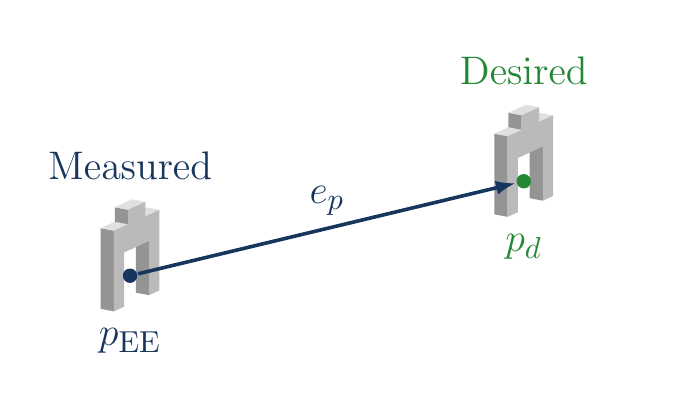
\begin{tikzpicture}[font=\fontsize{15}{18}\selectfont,
 >={Latex[length=2.5mm,width=1.8mm]}]
\path[use as bounding box] (0,0) rectangle (8,4.4);
\coordinate (M) at (1.3,1.25);
\coordinate (D) at (6.3,2.45);
\begin{scope}[shift={(M)},scale=.8]\PoseGripper\end{scope}
\begin{scope}[shift={(D)},scale=.8]\PoseGripper\end{scope}
\draw[->,measured,line width=1.3pt,shorten >=3pt,shorten <=3pt]
 (M)--(D) node[midway,above=3pt,fill=white,inner sep=1pt] {$e_p$};
\fill[measured] (M) circle (2.6pt);
\fill[desired] (D) circle (2.6pt);
\node[measured,anchor=north] at (1.3,.7) {$p_{\mathrm{EE}}$};
\node[desired,anchor=north] at (6.3,1.9) {$p_d$};
\node[measured] at (1.3,2.65) {Measured};
\node[desired] at (6.3,3.85) {Desired};
\end{tikzpicture}
\end{document}
